\subsection*{SARS}

\begin{table}[H]
    \begin{center}
      \begin{tabular}{@{}rlrl@{}}
        \toprule
        \multicolumn{4}{c}{\bf{Parameters values}}
        \\
        \midrule
        $\beta$
          & \num{0.2}
          & $d_1$, $d_2$
          & \num{0.0079}, \num{0.0337}
        \\
        $\varepsilon_E$, 
        $\varepsilon_Q$,
        $\varepsilon_J$
          & \num{0.3}, \num{0.0}, \num{0.1}
          &
          $k_1$, $k_2$ 
          & 
            \num{0.1},
            \num{0.125}
          \\
        $\mu$
          & \num{0.000034}
        \\
        $\Lambda$
          & $\mu N$
        \\
        $p$
          & \num{0.0}
        \\
        $\sigma_1$, $\sigma_2$
          & \num{0.0337}, \num{0.0386}
          && \multicolumn{1}{c}{\bf{Initial conditions}}
        \\
        \cmidrule{4-4}
          &&& $S(0)=\num{12e6}$, $E(0)=1565$,
         \\
        $t_f$
          & $\SI{1.0}{year}$
          && $Q(0)=292$, $I(0)=\num{695}$,
        \\
        Step size
        & $dt=\SI{1.0}{day}$
        && $J(0)=\num{326}$, $R(0)=\num{20}$
        \\
        $u_i$ bounds
          & \num{.05}, \num{0.5}
        \\
        $B_1$, $B_2$, $B_3$, $B_4$
        & \num{1.0}, \num{1.0}, \num{1.0}, \num{1.0}
        \\
        $C_1$, $C_2$
        & \num{300}, \num{600}
        \\
        \bottomrule
      \end{tabular}
     \caption{Parameter description for the SARS model
     \eqref{eqn:sars_model}.}
     \label{tbl:sars_table}
     \end{center}
\end{table}

\begin{figure}[H]
  \centering
  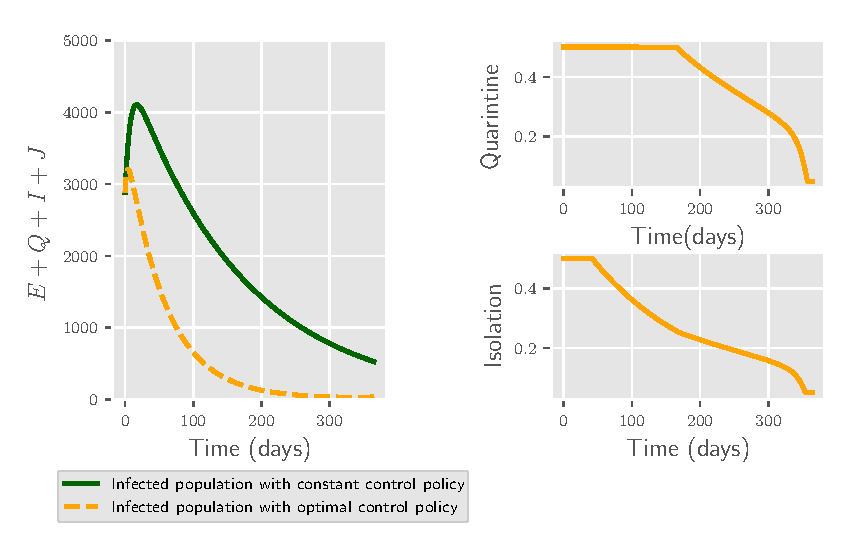
\includegraphics{Figures/figure_1_sars}
  \caption{}
  \label{fig:figure1sars}
\end{figure}

\begin{figure}[H]
  \centering
  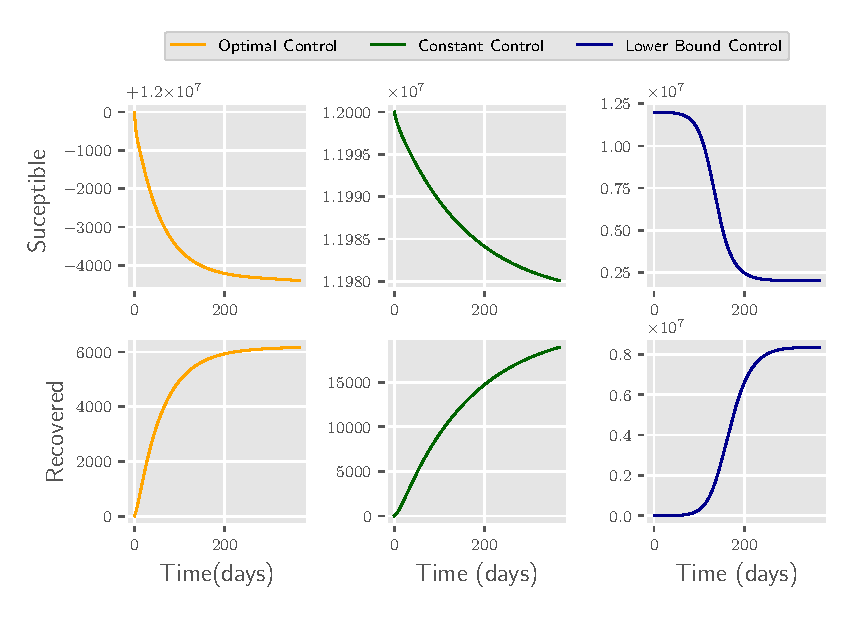
\includegraphics{Figures/figure_2_sars}
  \caption{}
  \label{fig:figure2sars}
\end{figure}

\begin{figure}[H]
  \centering
  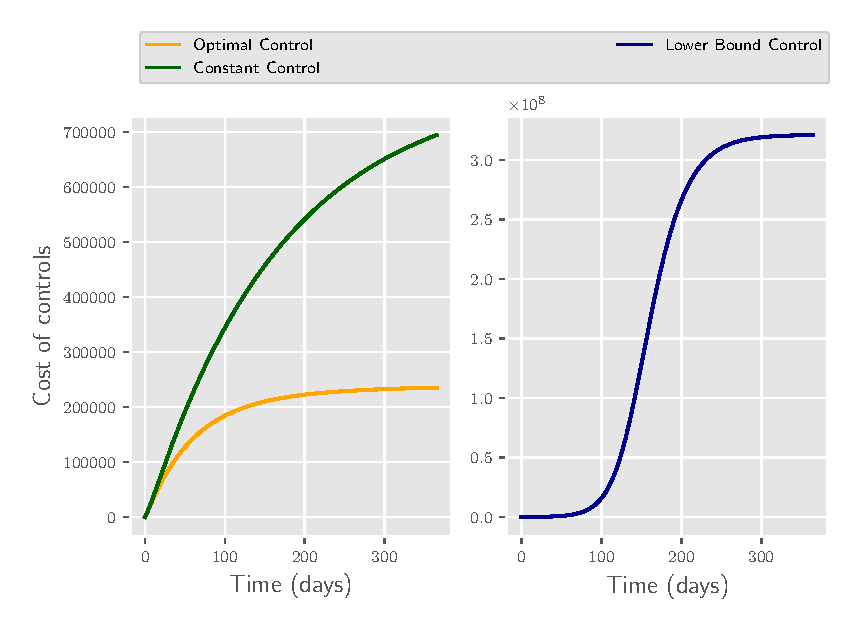
\includegraphics{Figures/figure_3_sars}
  \caption{}
  \label{fig:figure3sars}
\end{figure}